% !TeX program = xelatex
% !TeX encoding = UTF-8
% Template and editable FIM/NMG diagrams reused from beamer_v1.3.
\documentclass[aspectratio=1610]{ctexbeamer}
\usepackage{amsmath,amssymb,bm,array,booktabs,tabularx,listings,tikz}
\usetikzlibrary{arrows.meta,positioning,calc,shapes.geometric}
%%%%%%%%%%%%%%%%%%%%%%%%%%%%%%%%%%%
%% DO NOT CHANGE

\usetheme{default}
\useinnertheme{circles}
\useoutertheme{infolines}
\usefonttheme{serif}

\usepackage{etoolbox}

%% T for navigation symbols
%%\setbeamertemplate{navigation symbols}{}

%% T for header
%% \setbeamertemplate{headline}{%
%%   \leavevmode%
%%   \ifdefempty{\insertsubsectionhead}{
%%     \begin{beamercolorbox}[wd=0.99\paperwidth,ht=2.25ex,dp=1ex,center]{section in head/foot}%
%%       % \hbox to .5\paperwidth{\hfil\insertsectionhead\hfil}
%%       \insertsectionhead
%%     \end{beamercolorbox}%
%%   }{
%%     \begin{beamercolorbox}[wd=.44\paperwidth,ht=2.25ex,dp=1ex,right]{section in head/foot}%
%%       % \hbox to .5\paperwidth{\hfil\insertsectionhead\hfil}
%%       \insertsectionhead
%%     \end{beamercolorbox}%
%%     \begin{beamercolorbox}[wd=.1\paperwidth,ht=2.25ex,dp=1ex,center]{section in head/foot}%
%%       % \hbox to .5\paperwidth{\hfil\insertsectionhead\hfil}
%%       -
%%     \end{beamercolorbox}%
%%     \begin{beamercolorbox}[wd=.44\paperwidth,ht=2.25ex,dp=1ex,left]{subsection in head/foot}%
%%       % \hbox to .5\paperwidth{\hfil\insertsubsectionhead\hfil}
%%       \insertsubsectionhead
%%     \end{beamercolorbox}
%%   }%
%% }

%% T for frame title
\setbeamertemplate{frametitle}{%
  \usebeamerfont{frametitle}\insertframetitle\strut%
  \vskip-0\baselineskip%
  \leaders\vrule width .95\paperwidth\vskip1pt%
  \vskip0pt%
  \nointerlineskip
}

%% T for footer
\setbeamercolor{footlinecolor}{fg=cyan,bg=green}
\setbeamercolor{author in head/foot}{fg=blue}

\setbeamertemplate{footline}{%
  \leavevmode%
  \hbox{%
  \begin{beamercolorbox}[wd=.26\paperwidth,ht=2.25ex,dp=1ex,left]{author in head/foot}%
    \hspace*{2ex}\usebeamerfont{author in head/foot} NUAA
  \end{beamercolorbox}%
  \begin{beamercolorbox}[wd=.50\paperwidth,ht=2.25ex,dp=1ex,center]{author in head/foot}%
    \usebeamerfont{title in head/foot}HyMoS-Baltamatica
  \end{beamercolorbox}%
  \begin{beamercolorbox}[wd=.24\paperwidth,ht=2.25ex,dp=1ex,right]{date in head/foot}%
    \usebeamerfont{date in head/foot}

    \insertframenumber/\inserttotalframenumber\hspace*{2ex}
  \end{beamercolorbox}}%
  \vskip0pt%
}
%%%%%%%%%%%%%%%%%%%%%%%%%%%%%%%%%%%%%%%%%%%%%%%%

\setbeamertemplate{navigation symbols}{}
\hypersetup{unicode=true,colorlinks=true,urlcolor=blue,linkcolor=blue}
\setbeamersize{text margin left=0.55cm,text margin right=0.55cm}
\setbeamerfont{frametitle}{size=\large}
\setbeamerfont{institute}{size=\normalsize}
\newcommand{\Kn}{\mathrm{Kn}}
\newcommand{\bbf}{\boldsymbol f}
\newcommand{\bu}{\boldsymbol u}
\newcommand{\bq}{\boldsymbol q}
\newcommand{\bsigma}{\boldsymbol\sigma}
\newcolumntype{Y}{>{\raggedright\arraybackslash}X}
\newcommand{\refline}[1]{\par\vfill{\fontsize{7}{8.5}\selectfont\color{gray!85}#1}}
\newcommand{\subhead}[1]{\par\noindent{\color{structure.fg}\bfseries #1}\par\smallskip}
\lstset{basicstyle=\ttfamily\footnotesize,columns=fullflexible,keepspaces=true,
  breaklines=true,showstringspaces=false,frame=none,backgroundcolor=\color{gray!7},
  xleftmargin=4pt,xrightmargin=4pt,aboveskip=6pt,belowskip=6pt}
% Original styles used by the FIM diagram.
\tikzstyle{start} = [rectangle, draw, fill=pink!20,
text width=8em, text centered, rounded corners, minimum height=5em]
\tikzstyle{Euler} = [rectangle, draw, fill=blue!20,
text width=8em, text centered, rounded corners, minimum height=5em]
\tikzstyle{Moment} = [rectangle, draw, fill=yellow!20,
text width=8em, text centered, rounded corners, minimum height=5em]
\tikzstyle{line} = [draw, -stealth, line width=2pt]
\title{HyMoS-Baltamatica}
\subtitle{\texorpdfstring{一维稳态 Boltzmann--BGK 方程求解插件\\[0.4em]
\normalsize B3\quad 自选开源库插件开发}{一维稳态 Boltzmann--BGK 方程求解插件}}
\author{\texorpdfstring{团队成员：刘盛琦、陈升光、疏凌云\\[0.5em]指导教师：胡志成}{刘盛琦、陈升光、疏凌云；指导教师：胡志成}}
\institute{南京航空航天大学}
\date{\small v1.0.2}
\begin{document}

\begin{frame}[plain]
\titlepage
\end{frame}

\begin{frame}{选型依据}
\textbf{HyMoS（Hyperbolic Moment Solver）}采用矩方法求解气体动理学方程。插件将其一维稳态求解能力接入北太天元。
\par\vspace{0.3cm}
\begin{columns}[T,onlytextwidth]
\begin{column}{0.49\textwidth}
\subhead{算法特点}
\begin{itemize}
\setlength\itemsep{0.6em}
\item 局部 Hermite 展开截断至 $M$ 阶，经双曲正则化描述非平衡输运。
\item FIM 交替更新矩系统和宏观子系统，面向近连续流域的稳态计算。
\item NMG 通过粗网格校正加速收敛，支持改变网格、矩阶数及求解配置。
\end{itemize}
\end{column}
\begin{column}{0.47\textwidth}
\subhead{接入价值}
在北太天元内完成参数配置、后台求解、数组分析和绘图，复用其原生界面与工作区。
\par\vspace{0.45cm}
\subhead{应用场景}
面向微机电系统气体薄膜及近似平行间隙，分析壁面运动引起的剪切、温差传热及耦合效应，为气体阻力和传热参数筛选提供计算依据。
\end{column}
\end{columns}
\refline{Cai and Li, SIAM J. Sci. Comput. 32 (2010), 2875--2907; Cai, Fan and Li, CPAM 67 (2014), 464--518.\\
Cercignani, \textit{Slow Rarefied Flows: Theory and Application to Micro-Electro-Mechanical Systems}, 2006.}
\end{frame}

\begin{frame}{Boltzmann--BGK 模型}
\small
无外力 BGK 方程及局部 Maxwell 分布为
\[
\frac{\partial f}{\partial t}+\boldsymbol\xi\cdot\nabla_{\boldsymbol x}f
=\bar\nu(f^M-f),\qquad
f^M=\frac{\rho}{m_*(2\pi\theta)^{3/2}}
\exp\!\left(-\frac{|\boldsymbol\xi-\bu|^2}{2\theta}\right).
\]
$f=f(t,\boldsymbol x,\boldsymbol\xi)$ 为分子分布函数，$\boldsymbol\xi\in\mathbb R^3$。
$\rho,\bu,\theta$ 分别表示密度、平均速度、温度变量，$m_*$ 为单分子质量。
\par\vspace{0.22cm}
\subhead{插件中的一维稳态模型}
流动仅沿壁面法向 $x_1$ 变化，分子速度保留三个分量。
\[
\xi_1\frac{\partial f}{\partial x_1}=\bar\nu(f^M-f),\qquad
\bar\nu=\sqrt{\frac{\pi}{2}}\frac{\rho\theta^{1-\omega}}{\Kn},\quad\omega=0.81.
\]
\begin{center}
\renewcommand\arraystretch{1.2}
\begin{tabular}{lll}
\toprule
工况 & 壁面条件 & 主要输运过程\\
\midrule
Couette & 同温，切向壁速不同 & 剪切及黏性加热\\
Fourier & 不同温，切向壁速相同 & 温差传热\\
Couette--Fourier & 壁温、切向壁速均不同 & 剪切传热耦合\\
\bottomrule
\end{tabular}
\end{center}
两壁采用完全漫反射边界。
\refline{Bhatnagar, Gross and Krook, Phys. Rev. 94 (1954), 511--525.}
\end{frame}

\begin{frame}{快速迭代矩方法（FIM）}
\small
FIM（fast iterative moment method）交替求解高阶矩系统（HMS）和流体力学子系统（HEs），以应力及热流闭合宏观方程，再回代密度、速度和温度。
\begin{center}
\begin{tikzpicture}[node distance = 2cm, auto, scale=0.7, transform shape]
			% Place nodes
			\node [start] (init) {准备$\bbf$的初值};
			\node [Moment, right of=init, node distance=4.5cm] (moment-1) {通过求解HMS更
				新$\bbf$, 迭代步数$n=1$};
			\node [Euler, below of=moment-1, node distance=3cm] (euler-1)
			{通过求解HEs更新$\rho$, $\bu$, 和 $\theta$};
			\node [Moment, right of=moment-1, node distance=4.75cm] (moment-2) {通过求解
				HMS更新$\bbf$, 迭代步数$n=2$};
			\node [Euler, below of=moment-2, node distance=3cm] (euler-2)
			{通过求解HEs更新$\rho$, $\bu$, 和 $\theta$};
			\node [right of = moment-2, node distance=3.5cm] (ellipsis) {$\cdots$};
			\path [line] (init) -- (moment-1);
			\path [line, blue] (moment-1) -- (moment-2);
			\path [line, blue] (moment-2) -- (ellipsis);
			\path [line, red, line width=1.4pt, align=center] (moment-1) -- node
			[right=0pt] {\small $\rho$, $\bu$, $\theta$, \\ \small $\bsigma$, $\bq$, BC}
			(euler-1);
			%\path [line, gray, align=center] (euler-1.east) to [out=0,in=180]
			\path [draw, gray, line width=1.4pt, align=center] (euler-1.east) to [out=0,
			in=180]
			node[right] {\small $\rho$, $\bu$, $\theta$} ($(moment-2.west)-(0.25cm,0)$);
			\path [line, red, line width=1.4pt, align=center] (moment-2) -- node
			[right=0pt] {\small $\rho$, $\bu$, $\theta$, \\ \small $\bsigma$, $\bq$, BC}
			(euler-2);
			% \path [line, gray, align=center] (euler-2.east) to [out=0,in=180]
			\path [draw, gray, line width=1.4pt, align=center] (euler-2.east) to [out=0,
			in=180]
			node[right] {\small $\rho$, $\bu$, $\theta$} ($(ellipsis.west)-(0.25cm,0)$);
		\end{tikzpicture}
\end{center}
\par\vspace{-0.18cm}
\begin{center}
\renewcommand\arraystretch{1.05}
\begin{tabular}{lll}
\toprule
配置 & 高阶矩系统 & 流体力学子系统\\
\midrule
FIM-1 & 显式 Euler & 显式 Euler\\
FIM-2 & IMEX & 显式 Euler\\
FIM-3 & IMEX-SGS & SGS\\
\bottomrule
\end{tabular}
\end{center}
{\footnotesize IMEX：输运项显式、碰撞项隐式。SGS：对称 Gauss--Seidel 扫掠。BC：相容的宏观边界条件。}
\refline{Li, Wang and Hu, A fast iterative moment method for near-continuum gas flows, Comput. Fluids 311 (2026), 107031.}
\end{frame}

\begin{frame}{非线性多重网格方法（NMG）}
NMG（nonlinear multigrid）在空间粗网格上计算校正，处理细网格中衰减缓慢的误差。各层保持相同矩阶数，以 FIM 为光滑子。
\par\vspace{0.3cm}
\begin{columns}[T,onlytextwidth]
\begin{column}{0.49\textwidth}
\centering
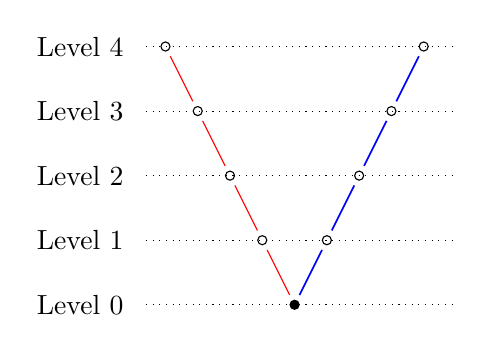
\begin{tikzpicture}[scale=0.82]
				\foreach \y in {0,1,2,3,4}
				{
					\draw[dotted] (0.2,\y)--(5,\y);
					\node[anchor=east] at (0,\y)
					{Level $\y$};
				}

				\draw (2.5,0) node (c1) {};
				\draw[fill] (c1) circle [radius=2pt];

				\foreach \x/\xtext in {2/1,3/2}
				{
					\draw (\x,1) node (c1x\xtext) {};
					\draw (c1x\xtext) circle [radius=2pt];
				}

				\foreach \x/\xtext in {1.5/1,3.5/2}
				{
					\draw (\x,2) node (c2x\xtext) {};
					\draw (c2x\xtext) circle [radius=2pt];
				}

				\foreach \x/\xtext in {1/1,4/2}
				{
					\draw (\x,3) node (c3x\xtext) {};
					\draw (c3x\xtext) circle [radius=2pt];
				}

				\foreach \x/\xtext in {0.5/1,4.5/2}
				{
					\draw (\x,4) node (c4x\xtext) {};
					\draw (c4x\xtext) circle [radius=2pt];
				}

				\draw[red]
				(c1)--(c1x1)--(c2x1)--(c3x1)--(c4x1);

				\draw[blue,semithick]
				(c1)--(c1x2)--(c2x2)--(c3x2)--(c4x2);
			\end{tikzpicture}
\par\smallskip{\small $V$-cycle}
\par\medskip
{\footnotesize
\tikz[baseline=-0.5ex]\draw (0,0) circle[radius=1.5pt];\ FIM 光滑\quad
\tikz[baseline=-0.5ex]\draw[fill] (0,0) circle[radius=1.5pt];\ 最粗层求解\\[0.5em]
\tikz[baseline=-0.5ex]\draw[red] (0,0)--(0.3,0);\ 限制\qquad
\tikz[baseline=-0.5ex]\draw[blue,semithick] (0,0)--(0.3,0);\ 延拓}
\end{column}
\begin{column}{0.46\textwidth}
\small
\subhead{一次循环}
\begin{enumerate}
\setlength\itemsep{0.7em}
\item 细网格执行 FIM 前光滑。
\item 将近似解及残差限制到粗网格，求解粗网格校正。
\item 将校正逐层延拓到细网格，执行 FIM 后光滑。
\end{enumerate}
\par\vspace{0.25cm}
\subhead{界面配置}
\texttt{single}：单网格 FIM。\\[0.4em]
\texttt{nmg}：FIM 光滑及粗网格校正，支持 V、W、F 循环。
\end{column}
\end{columns}
\refline{Hu and Li, A nonlinear multigrid steady-state solver for 1D microflow, Comput. Fluids 103 (2014), 193--203.}
\end{frame}

\begin{frame}{插件架构}
\begin{columns}[T,onlytextwidth]
\begin{column}{0.53\textwidth}
\centering
\begin{tikzpicture}[
module/.style={draw=black!55,fill=blue!3,align=center,text width=6.0cm,
minimum height=0.9cm,font=\footnotesize,inner sep=4pt},
request/.style={-{Stealth[length=1.5mm]},draw=blue!70!black},
response/.style={-{Stealth[length=1.5mm]},dashed,draw=black!65}]
\node[module] (host) at (0,0) {\textbf{北太天元交互层}\\参数表单、运行监视、结果绘图};
\node[module] (adapter) at (0,-1.55) {\textbf{SDK 适配层}\quad\texttt{main.so}\\函数注册、任务句柄、数据转换、导出};
\node[module,fill=green!4] (engine) at (0,-3.1) {\textbf{任务引擎}\\输入校验及快照、后台线程、进度记录};
\node[module,fill=green!4] (solver) at (0,-4.65) {\textbf{数值求解器}\\矩离散、壁面边界、FIM、NMG};
\foreach \a/\b in {host/adapter,adapter/engine,engine/solver}{
\draw[request] ([xshift=-16mm]\a.south)--([xshift=-16mm]\b.north);
\draw[response] ([xshift=16mm]\b.north)--([xshift=16mm]\a.south);}
\end{tikzpicture}
\par\medskip{\footnotesize 实线：配置及控制\qquad 虚线：状态及结果}
\end{column}
\begin{column}{0.43\textwidth}
\small
\subhead{技术栈}
\noindent\begin{tabularx}{\textwidth}{@{}lY@{}}
M 语言 & 原生 \texttt{uifigure} 和绘图\\[0.5em]
C++11 & SDK 适配、线程及原子变量\\[0.5em]
OpenMP & 数值计算并行\\[0.5em]
CMake & 构建共享库及插件\\
\end{tabularx}
\par\vspace{0.35cm}
\subhead{任务及数据}
任务引擎和求解器封装在\linebreak
\texttt{libhymos.so.5} 中。\\[0.65em]
提交时保存输入快照，后台线程执行计算。适配层将场量复制为宿主结构体和列主序数组。\\[0.65em]
停止请求在迭代检查点生效，卸载前等待工作线程退出。
\end{column}
\end{columns}
\end{frame}

\begin{frame}[fragile]{安装部署}
\small
\begin{columns}[T,onlytextwidth]
\begin{column}{0.54\textwidth}
\subhead{预编译包}
运行环境：Ubuntu 24.04 x86\_64（含 WSL2），北太天元 2025 Linux 版。
\begin{enumerate}
\setlength\itemsep{0.6em}
\item 从项目 Releases 下载 v1.0.2 Linux 包并解压。
\item 将完整 \texttt{HyMoS-Baltamatica/} 目录放入宿主 \texttt{plugins/} 目录。
\item 在北太天元加载插件并打开参数窗口。
\end{enumerate}
\begin{lstlisting}
load_plugin('HyMoS-Baltamatica');
hymos_setup('1D');
\end{lstlisting}
\end{column}
\begin{column}{0.42\textwidth}
\subhead{依赖及构建}
发布包内含求解库、脚本、模板和算例。系统提供 C/C++ 及 OpenMP 运行库（\texttt{libgomp1}）。
\par\vspace{0.35cm}
修改源码后，可使用北太天元 SDK、GCC 9.5 和 CMake 重新构建：
\begin{lstlisting}
bash scripts/build.sh
\end{lstlisting}
源码构建使用 Eigen、Boost、MPI、FFTW、oneTBB 开发包。完整安装命令见 \texttt{docs/BUILD.md}。
\end{column}
\end{columns}
\par\vfill
{\footnotesize 下载：\url{https://github.com/Liuyong2355/HyMoS-Baltamatica/releases}}
\end{frame}

\begin{frame}{图形界面配置}
\begin{columns}[T,onlytextwidth]
\begin{column}{0.65\textwidth}
\centering
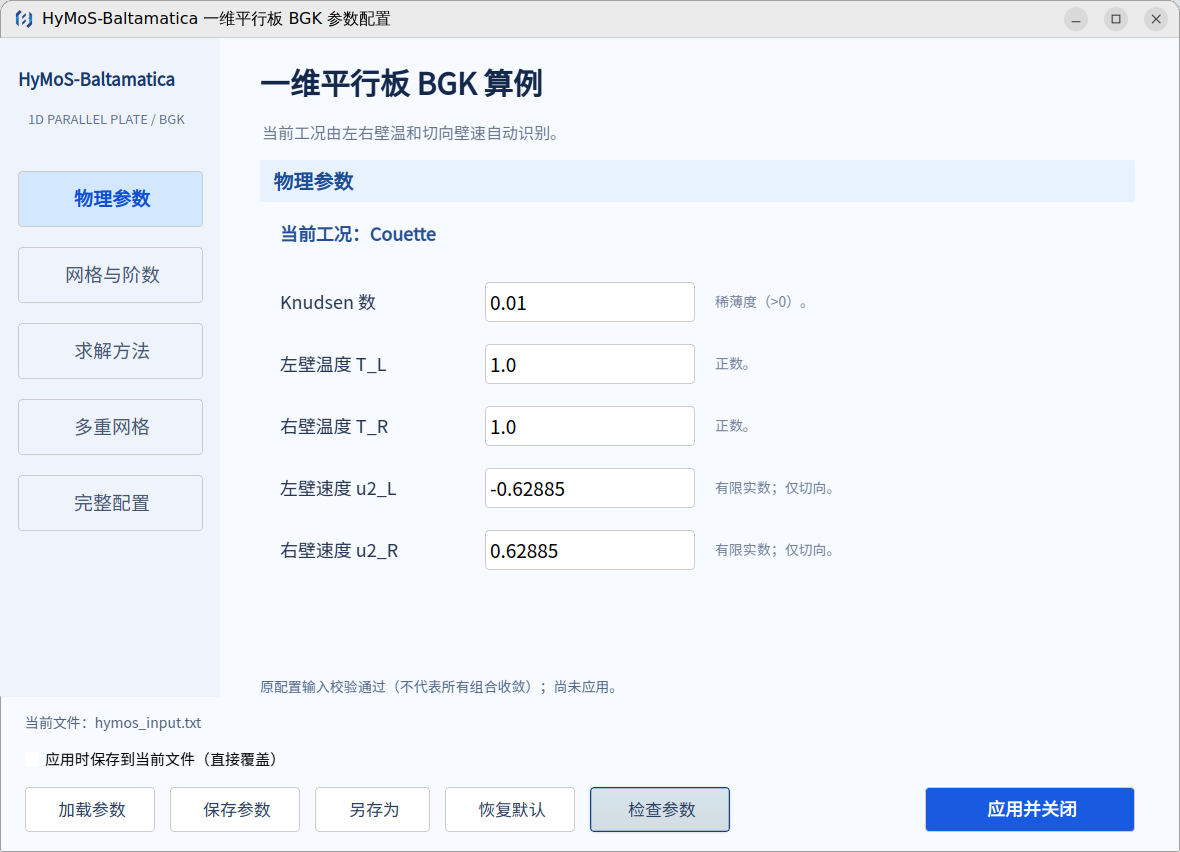
\includegraphics[width=\linewidth,height=6.9cm,keepaspectratio]{figures/parameter-window.png}
\end{column}
\begin{column}{0.32\textwidth}
\small
\subhead{配置顺序}
\begin{enumerate}
\setlength\itemsep{0.65em}
\item 物理参数：$\Kn$、两壁温度及切向速度。
\item 网格阶数：$N_1\ge8$，矩阶数 $M$。
\item 求解方法：FIM-1/2/3，\texttt{single/nmg}，建议 1--4 线程。
\item NMG：最粗网格尺寸、光滑次数、V/W/F 循环。
\end{enumerate}
\par\vspace{0.25cm}
在随包模板上修改，也可直接填写界面。检查参数通过后，点击“应用并关闭”。
\end{column}
\end{columns}
\end{frame}

\begin{frame}[fragile]{计算运行}
\begin{lstlisting}
hymos_run();
\end{lstlisting}
\small
按已应用的参数提交计算，任务对象保存为 \texttt{hymos\_task}。前台显示状态、迭代数、残差及耗时，后台线程执行求解。
\par\vspace{0.3cm}
\renewcommand\arraystretch{1.4}
\noindent\begin{tabularx}{\textwidth}{@{}p{0.56\textwidth}Y@{}}
\toprule
调用 & 作用\\
\midrule
\texttt{s = hymos\_status(hymos\_task)} & 查询状态、残差及耗时\\
\texttt{hymos\_monitor(hymos\_task)} & 继续显示运行进度\\
\texttt{hymos\_stop(hymos\_task)} & 请求在安全迭代检查点停止\\
\texttt{s = hymos\_wait(hymos\_task,10)} & 等待结束或 10 秒超时\\
\bottomrule
\end{tabularx}
\par\vspace{0.3cm}
Ctrl+C 可中断前台监视，后台计算继续。\texttt{converged} 表示达到残差容差，\texttt{iteration\_limit} 表示达到迭代上限。
\par\vfill
{\footnotesize 接口名称、参数和返回值详见 \texttt{docs/API.md}。}
\end{frame}

\begin{frame}[fragile]{结果分析}
\begin{columns}[T,onlytextwidth]
\begin{column}{0.49\textwidth}
\centering
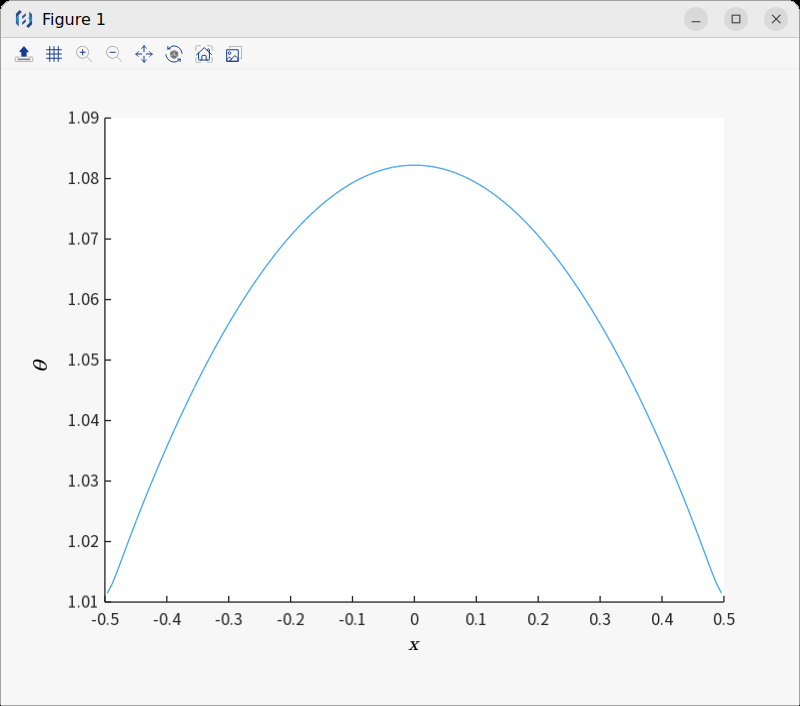
\includegraphics[width=\linewidth,height=5.8cm,keepaspectratio]{figures/couette-temperature.png}
\par\smallskip{\small 北太天元绘制的 Couette 温度曲线}
\end{column}
\begin{column}{0.48\textwidth}
\begin{lstlisting}
r = hymos_result(hymos_task);
plot(r.x, r.temperature);
files = hymos_export(hymos_task);
\end{lstlisting}
\small
\subhead{结构化结果}
\texttt{r} 包含坐标、密度、三分量速度、温度、应力矩、热流及残差历史，可继续使用宿主数组运算。
\par\vspace{0.3cm}
\subhead{导出数据}
\texttt{files} 返回导出路径。输出包含场量 CSV、残差 CSV 及运行信息，同时保留输入快照和分布展开数据。
\end{column}
\end{columns}
\end{frame}

\begin{frame}[fragile]{随包算例}
\small
\renewcommand\arraystretch{1.35}
\noindent\begin{tabularx}{\textwidth}{@{}p{0.34\textwidth}YY@{}}
\toprule
模板 & 工况 & 功能检查\\
\midrule
\texttt{couette.txt} & 壁面剪切 & 收敛及壁速特征\\
\texttt{fourier.txt} & 温差传热 & 温度及热流场量\\
\texttt{couette\_fourier.txt} & 剪切传热耦合 & 结构化结果及导出\\
\bottomrule
\end{tabularx}
\par\vspace{0.25cm}
\subhead{宿主集成检查}
以源码仓库为当前目录，在已加载插件的北太天元中执行：
\begin{lstlisting}
addpath('tests/baltamatica');
hymos_smoke_tests('examples/ParallelPlate1D');
\end{lstlisting}
检查三种工况的收敛、场量和导出，并覆盖最小网格及无效输入。
\par\vspace{0.22cm}
\subhead{源码回归}
\texttt{tests/library/} 提供配置读取、内存/CLI 结果、FIM/NMG、异步执行及停止等测试。构建脚本自动运行 CTest。
\end{frame}

\begin{frame}{项目资料}
\subhead{公开仓库}
\url{https://github.com/Liuyong2355/HyMoS-Baltamatica}
\par\vspace{0.25cm}
\small
\noindent\begin{tabularx}{\textwidth}{@{}p{0.31\textwidth}Y@{}}
\toprule
资料 & 位置\\
\midrule
源码、构建脚本、发布包 & 仓库及 Releases（v1.0.2）\\
技术文档、接口、构建说明 & \texttt{docs/}\\
算例及测试源码 & \texttt{examples/}、\texttt{tests/}\\
讲解视频 & \texttt{submission/}\\
\bottomrule
\end{tabularx}
\par\vspace{0.25cm}
项目采用 MIT 许可证，第三方组件保留各自许可及署名，详见 \texttt{THIRD\_PARTY\_NOTICES.md}。
\par\vspace{0.4cm}
\subhead{致谢}
感谢新加坡国立大学蔡振宁教授提供 NRxx 代码。\\[0.4em]
联系邮箱：\href{mailto:matcz@nus.edu.cn}{\nolinkurl{matcz@nus.edu.cn}}。
\par\vfill
{\footnotesize 图形界面借助 AI 辅助开发，技术文档及演示文稿借助 AI 整理，演示视频借助 AI 剪辑。}
\end{frame}
\end{document}
